

\section{Experimental Reconstruction of the Zebrafish Early Development }
\begin{figure}
\begin{center}
\includegraphics[width=0.75\textwidth]{../../images/experimental_science/experimental_science_cleaner_focus_reconstruction_live.png}
\end{center}
\caption{\textbf{Situation of Chapter 7 in the methodological workflow.}}
\label{experimental_science_experimental_science_cleaner_focus_reconstruction_live}
\end{figure}

\subsection{Bioemergences Reconstruction Workflow  }
\begin{figure}
\begin{center}
\includegraphics[width=0.9\textwidth]{../../images/Reconstruction/bioemergences/c_elegans_lineage_kipreos_2005.png}
\end{center}
\caption{Cell lineage from the \textit{Caenorhabditis elegans} embryonics and larval stages from Kipreos, E.T., 2005. C. elegans cell cycles: invariance and stem cell divisions. Nature reviews Molecular cell biology, 6(10), pp.766–776. \cite{Kipreos:2005im}}
\label{bioemergences_c_elegans_lineage_kipreos_2005}
\end{figure}

\textbf{Objective}: Reconstruction of the complete cell lineage tree of the Zebrafish early development. The lineage tree is augmented by the spatial coordinates and the shape of the cells (3D+time digital embryo) and by the quantification of various gene expression of the cells (Atlas of genetic expression). 

  The reconstruction task is a very tedious one and semi or complete automation is the only solution to tackle such an enormous lineage tree. 

  In this section, we will introduce the past and current strategies originated by the European project Embryomics and Bioemergences and pursued the Bioemergences team. This section is divided as the following: 
\begin{itemize}
	\item 1. Embryo Preparation and Acquisition
	\item 2. Cell lineage reconstruction workflow
\begin{itemize}
	\item 1. Workflow
	\item 2. Visualization / Correction
	\item 3. Validation
\end{itemize}
	\item 3. Post-processing / Higher level reconsruction / Exploitation
	\item 4. 4D atlas of gene expression
	\item 5. \textit{In toto} cell lineage
\end{itemize}    Discussion ->Prototype   

\textbf{Various challenges}: in addition to the challenges to design the aforementioned reconstruction strategy, various challenges arises from the limitation of the current imaging setups.  

  Workflow inputs: raw data 
\begin{itemize}
	\item The workflow is efficient if the spatio-temporal resolution of the raw data produced by the microscope device satisfies some required signal properties.
\begin{itemize}
	\item spatially, the signal-to-noise ratio must be limited and the local resolution of the    
	\item temporally, the difference between two images of the same region must be small enough as the image must not move too much.
\end{itemize}
\end{itemize}

  Unfortunately, these two requirements are antagonists and a trade-off must be found 

  Solution:  

  Most of the improvement must be applied in the imaging technique area but, given their limitations, algorithmic bandages must be designed to overcome them.  

  We distinguish between the fundamental reconstruction workflow which, in its idealized form, will remain relevant for a long time (pas terrible XXXX) and the modules which are subjugated to the limits of microscope performance (signal and scale of the raw data) and will become obsolete as soon as the microscope improves. \textit{in toto}  error-less: automated vs manual (introduire application thierry),  channel limitation    The prototype                     
\begin{figure}
\begin{center}
\includegraphics[width=0.6\textwidth]{../../images/Reconstruction/bioemergences/FigureWorkflow/Workflow2.png}
\end{center}
\caption{Workflow of reconstruction of the cell lineage}
\label{bioemergences_FigureWorkflow_Workflow2}
\end{figure}

  review of embryogenesis reconstruction : 

  Keller, P.J. et al., 2008. Reconstruction of zebrafish early embryonic development by scanned light sheet microscopy. Science, 322(5904), pp.1065–1069. \cite{Keller:2008km}

  Giurumescu, C.A. et al., 2012. Quantitative semi-automated analysis of morphogenesis with single-cell resolution in complex embryos. Development, 139(22), pp.4271–4279. \cite{Giurumescu:2012ej}

  example reconstruction: 

  Xiong, Y. amp;glesias, P.A., 2010. Tools for analyzing cell shape changes during chemotaxis. Integrative Biology, 2(11-12), pp.561–567. \cite{Xiong:2010ck}

  review -> Khairy, K. amp;eller, P.J., 2011. Reconstructing embryonic development P. M. Kulesa, M. E. Dickinson, amp;.-K. Hadjantonakis, eds. genesis, 49(7), pp.488–513. \cite{Khairy:2011ht}

\subsubsection{Embryo Preparation and Acquisition  }

  Embryo Preparation from paper methodo, à modifier: 

  Wild-type zebrafish embryos were injected at the one cell stage with 200pg mCherry/H2B RNA and 200pg eGFP-ras prepared from PCS2+ constructs [Moriyoshi, 1996 #35;Shaner, 2005 #29]. Although mCherry, unlike eGFP, bleached significantly through imaging, this colour combination was the best compromise allowing proper staining of the cell membranes for further segmentation. Injected embryos were raised at 28.5°C for the next 3 hours. Embryos were mounted in a 3cm Petri dish with a glass coverslip bottom, sealing a hole of 0.5mm at the Petri dish centre where a Teflon tore (ALPHAnov) with a hole of 780µm received the dechorionated embryo. The embryo was maintained and properly oriented by infiltrating around it 0.5% low melting point agarose (Sigma) in embryo medium [Westerfield, 2000 #36]. Temperature control in the room resulted in a temperature of about 26°C under the objective slightly slowing down development with respect to the standard 28.5°C developmental table [Kimmel, 1995 #11] (Table S1). After the imaging procedure, embryo morphology was checked under the dissecting binocular and the animal was raised for at least 24h to assess morphological defects. Embryo survival depends on total imaging duration, average laser power, and image acquisition frequency (or time step ∆t). 070418a and 070420a correspond to a standardised procedure with 50s < ∆t < 70s allowing 75-110 sections per time point for 10 hours with an average laser power of 80 mW delivered to the sample. Lowering the laser power to less than 60 mW and lengthening ∆t up to 3.5min allowed imaging embryos for more than 20 hours, then raising them until adulthood. These conditions were used for making up to 320 sections at 400Hz line scan rate (bidirectional scanning), or 200Hz to improve signal-to-noise ratio, as for the image data set 080322a shown in movie 1-3.  

  Image acquisition from paper methodo, à modifier: 

  Imaging was achieved with a Leica upright microscopes SP5 MLSM equipped with a 20/0.95NA W dipping lens objective (Olympus) or Leica 20/1NA W dipping lens objective. Axial resolution at the sample surface (1.5µm) was estimated by recording 3D images of 0.1 or 1µm fluorescent polystyrene beads (Invitrogen) at the surface of an agarose gel. Field size was 700x700 or 775x775 microns in x, y, 140µm in z for 070418a and 100µm in z for 070420a; voxel size was 1.37x1.37x1.37µm or 1.51x1.51x1.51µm. Simultaneous dual wavelength excitation with pulses at two different wavelengths (980 and 1030nm). At 1030 nm, pulsed laser beam (50Mhz, 200fs) was provided by a solid-state Ytterbium femtosecond oscillator (T-pulse 20, Amplitude Systèmes). At 980 nm, pulsed laser beam (80Mhz, 100fs) was provided by a Ti-Sapphire femtosecond oscillator (Mai Tai HP, Newport Spectra physics). Details of the optical bench are provided in supplementary material. Raw data visualisation was done using Amira software (Mercury Computer Systems).  

\subsubsection{Cell Lineage Reconstruction Workflow  }

\paragraph{Workflow}
\begin{figure}
\begin{center}
\includegraphics[width=0.8\textwidth]{../../images/Reconstruction/bioemergences/FigureWorkflow/Workflow2_lineage_only.png}
\end{center}
\caption{}
\label{bioemergences_FigureWorkflow_Workflow2_lineage_only}
\end{figure}

\subparagraph{Filtering}

  Raw data images are filtered with specific nonlinear geometrical PDEs called "Geodesic Mean Curvature Flow" (GMCF). In GMCF, the contrast-invariant flows achieved nonlinear multiscale analysis on scalar intensity functions in the voxel intensity histogram \cite{Rizzi:2007bz}\cite{Kriva:2010cs}.. This iterative strategy eliminate most of the noisy signal. 

\subparagraph{Cell identification}

  Once, the nuclei and membrane images have been filtered, the nuclear centers are detected by a nonlinear PDE-based multiscale strategy called "Flux-Based Level Set Center Detection" (FBLSCD). On the nuclei image, the FBSLSCD iteratively decreases the size of the nuclei signal until a given stopping condition is reached. The last remaining local maxima gives the position of the cell centers \cite{Frolkovic:2007ti}. 

\subparagraph{Shape Segmentation}
\begin{figure}
\begin{center}
\includegraphics[width=0.8\textwidth]{../../images/Reconstruction/bioemergences/segmentation/images_segmentation.png}
\end{center}
\caption{Top. Left. A triangle with subjective contour \cite{Sarti:2000jw}. Right. Evolution of the subjective surface technique towards the contour \cite{Sarti:2000jw}. Bottom. Segmentation of membrane with an uncomplete contour \cite{Zanella:2007vh}.}
\label{segmentation_images_segmentation}
\end{figure}

  The proper segmentation of both the surface of the cell membranes and cell nuclei is then performed from the position of the cell centers. The algorithm used is called the "Subjective Surface Technique" (SST) \cite{Sarti:2000jw}. For each cell, the segmentation is performed from the point of view of the center. The surface grows around it until it reaches an obstacle, the surface then deforms to adopt the shape of the surrounding signal. The key advantage of this technique is its ability to deal with the incomplete information of the image and still propose a hole-less segmentation.  

  The segmentation of the nuclei and membrane are used to automatically correct some errors in the center detection step. If two centers are detected but the segmentation provide the same subjective surface, the duplicated center. Similarly, segmentation are used to detect mitosis if two mitosis are inducing the same membrane. The information of a probable cell duplication is used by the following cell tracking algorithm. 

reference recente: Mosaliganti, K.R. et al., 2012. ACME: Automated Cell Morphology Extractor for Comprehensive Reconstruction of Cell Membranes R. F. Murphy, ed. PLoS Computational Biology, 8(12), p.e1002780. \cite{Mosaliganti:2012gj}

\subparagraph{Cell tracking}

  The cell tracking algorithm is the key module of this workflow. It relates temporally the identity of the cell in between time steps. From the initial cell population, these temporal links form a tree whose branches split when a cell divides. The tracking is build in three steps: 
\begin{itemize}
	\item an \textit{a priori} step which specifies the strong local constraints that restricts the list of putative links. The constraints are mainly the suppression of all putative links which relates cell which would have move above a given maximum distance and the number of daughter links.
	\item a central step which consists in minimizing a heuristic function which combines the information extracted from the processed images (center positions, large scale vector fields, segmentation) with a biophysical regularization constraint (see Kirkpatrick 1983 XXXX).
	\item an \textit{a posteriori} step which processes the obtained tree to minimize the number of false-positive and false-negative errors detected in the segmentation module.
\end{itemize}

\paragraph{Visualization / Correction}

  Moveit 

  A major challenge for the reconstruction of developing embryos is the design of tools adapted the handling of the produced data sets. 

  The specificity of these new kind of data (a mapping between a graph = lineage tree and various type of local cell data = morphological, positional, genetic expression...) make them mostly incompatible with existing data-handling software solution.    new type of phenomological   a new kind of digital specimen  original  augmented reconstructed phenomenology        dedicated tool for visualization and correction/validation of the reconstruction of developing embryos.      Necessité d'un outil qui répond à une double demande   Data visualization:   exhaustive visualization: from the raw data to the (cell centers + cell nuclear and membrane segmentation)  + and every intermediate data used in the workflow ?    multiscale: from the fields of microscopic data and the focus on local data     direct biological insight extraction:        fate mapping : avant non seulement flou, lien continu entre repere et injection    cell fate given by the lieneage    evolution of the cell proliferation rate    clonal population selection    origin polyclonal des organes:     exemple hors bioemergences -> lineage exploitation for stem cell studies (Simons, B.D. \& Clevers, H., 2011. Strategies for Homeostatic Stem Cell Self-Renewal in Adult Tissues. Cell, 145(6), pp.851–862. \cite{Simons:2011ec})  from Lombardot, B., 2010. Description intégrative des cinématiques de la structure embryonnaire : morphogenèse précoce du poisson zébré. Ecole Polytechnique EDX Paris.  "Inter^et de l'etude des destinees : L'etude des destinees est tres informative au premier abord sur la morphogenese embryonnaire. Les cartes de destinees et les lignages cellulaires indiquent ou vont les cellules et comment (dans le cas du lignage). Cependant ca n'est pas le seul inter^et de l'etude des destinees. Comme nous venons de le voir les destinees dans l'embryon peuvent dependre du lignage mais aussi d'une regulation de l'environnement. Les cartes de destinees ou les lignages ne donnent pas d'information directe sur la regulation, par contre, l'etude du lignage, les analyses clonales et leur association a des informations complementaires sur le comportement des cellules, leur activite biochimique et leur mode de division peuvent ^etre indicatifs d'une restriction du potentiel d'une cellule ou d'une population de cellules. L'analyse clonale (ie. l'analyse des descendants d'une cellule) permet de s'interroger sur le lignage qui permet la transformation observ ee : nombre de divisions, nombre de cycles cellulaires, distribution des types cellulaires, organisation spatiale des descendants [38]. L'etude de ces grandeurs permet de s'interroger sur l'activite specifique associee a la mise en place d'une structure. Si on etudie les caracteristiques d'un territoire presomptif au cours du temps, il pourrait ^etre possible de caracteriser la periode d'apparition des comportements specifiques a la descendance de la region. Indirectement il serait donc possible de distinguer les periodes auxquelles se font les restrictions du potentiel developpemental des cellules."                      Data modification:   The automated reconstruction workflow does not produce error-less reconstruction.    expliquer comment sont corrigées les centres, liens grace à l'interface  correction -> existence and position of cell centers, cell link between two consecutive time steps    Key points:   Mapping between the flat representation of the lineage tree and the 3D   Time controlling: backward and forward  Propagation of measures on a clonal, backward and forward   from papier methodo   Processing supervision, data annotation, validation, correction and analysis were performed with the Mov-IT interactive visualization software     

\paragraph{Validation}     Validation:   Manual validation versus automated validation    Manual validation: statistical analysis from the hand-corrected tracking links     "The tracking error rate was measured (make it only for shorter time) with the sampling procedure described in Figure 4d and Methods section. Altogether, over 15,000 links between the t and t+1 positions of cells have been manually checked at different time points. For the first 300 time steps (5h34 imaging, end of gastrulation) the total error rate is lower than 2%, i.e., more than 98% of the cells were correctly tracked (Figure 4d)."  False positives in nuclear detection were kept below 0.5% and were not the major source of tracking errors. About half of the tracking errors were identified as false trajectories (the tracking jumped from one cell trajectory at time t to another at time t+1) and the other half was false deaths (the tracking did not find the position of the cell at time t+1, and cell trajectory ended).     Automated validation : the salt and pepper strategy  "" Validation with the above sampling procedure remained a time consuming task. We however showed that similar data sets i.e. corresponding to the same developmental period, labelling and imaging conditions, provided similar results. Nevertheless, we looked for an automated validation strategy and came up with the following. Transplanting about one hundred cells between high stage and sphere stage [Kimmel, 1995 #11] from a donor embryo with double stained nuclei (H2B/mcherry through RNA injection into H2A/eGFP transgenic embryos) into a transgenic host with green nuclei [Pauls, 2001 #236] provided means to both assess our tracking performances in the context of the whole embryo cells tracking (the salt channel) and in the context of a small subpopulation of labelled nuclei (the pepper channel). We were able to show that tracking accuracy in the pepper channel is as good as the hand-made gold standard (gs) and that the automated comparison with either the gold standard or the automatically tracked pepper channel (lineage tree p) provided the same measurement for the “salt channel” tracking accuracy (Figure 5). Mappings mgs,p; mgs,s and ms,p (explain more)   identifying the same cell in both dataset were created. These mappings minimized the distance between matching cells. Cell i is catgoarized as false positive if i is in the set gs / Range(m[gs,p]) (Figure 4 b?), false negative if i is in p / Domain(m[gs,p]) (Figure 4 c?). An error in cell detection is defined as range(m[gs,p]) Δ domain(m[gs,p]).  We conclude about a tracking error if f(it+1)=jt and f(m(it+1)) != m(jt) where f is the predecessor function (Figure 4 d?).  There was no significant difference in errors’ categorization plots when the mappings Mgs,s and Ms,p were compared. The errors characterization done with two different evaluation methods, salt & paper and manually (figure 4), applied to the reconstruction of two individuals, showed similar numbers. The salt & pepper strategy allowed the fully automated evaluation of the reconstruction accuracy and errors’ categorization without manual intervention.  Provided that imaging labelling procedures and imaging set up allowed a third colour and channel, the salt and pepper strategy might be performed still preserving the membrane channel and the possibility to get measurements for cell shape.  ""      

\subsubsection{Post Processing and Exploitation  }

\textbf{Spatio-temporal cartography of the cell kinematics}

   Thèse Benoit -> Lombardot, B., 2010. Description intégrative des cinématiques de la structure embryonnaire : morphogenèse précoce du poisson zébré. Ecole Polytechnique EDX Paris. \cite{Lombardot:2010vd}

  On présente rapidement les mesures utilisées par Benoît M U ... en ensuite les cartes.  

   Ajouter mesures 
\begin{figure}
\begin{center}
\includegraphics[width=0.7\textwidth]{../../images/Reconstruction/these_lombardot/p93_texture_tensor.png}
\end{center}
\caption{Le tenseur de texture de la cellule i (jaune) peut ^etre vu comme une caracterisation geometrique de la forme du voisinage de i (A). Le tenseur de texture (vert) est proche de la covariance du voisinage de i (rouge) (B). Le tenseur de texture peut aussi ^etre interprete comme la covariance du voisinage symetrise de i. adapted from XXXXXX}
\label{these_lombardot_p93_texture_tensor}
\end{figure}
\begin{figure}
\begin{center}
\includegraphics[width=0.7\textwidth]{../../images/Reconstruction/these_lombardot/p94_texture_tensor_average.png}
\end{center}
\caption{En general, le tenseur de texture n'est pas defini pour une cellule mais pour une collection de cellules C (cellule dans le cercle jaune). Comme pour une representation "coarse grained" du milieu le tenseur de texture a la position X est defini par la moyenne des tenseurs de texture de chaque cellule de la region de mesure (cercle jaune) (a droite). En representant tous les liens impliques dans la mesure du tenseur de texture au point X (M(X)), on comprend bien que M(X) est une caracterisation moyenne de la forme des voisinages cellulaires dans la region de mesure autour de X.}
\label{these_lombardot_p94_texture_tensor_average}
\end{figure}
\begin{figure}
\begin{center}
\includegraphics[width=0.7\textwidth]{../../images/Reconstruction/these_lombardot/p98_texture_tensor_derivative.png}
\end{center}
\caption{La derivee de M traduit la description intuitive de l'evolution du voisinage d'une cellule. Le tenseur de texture de la cellule i (jaune) a t + dt est egale au tenseur de texture de i a t (M(t)) auquel trois contributions sont ajoutees : la premiere traduit la deformation continue des positions de cellules restant dans le voisinage de i (cellules bleues), la seconde traduit l'entree de cellules dans le voisinage (cellules rouges), enfin la derniere contribution correspond aux cellules sortant du voisinage (cellules vertes). Ces trois contributions correspondent respectivement aux tenseurs B(t), n_ +M+ et n_ M. Cette interpretation intuitive n'est valide que si le nombre de liens apparus est egal au nombre de liens disparus.}
\label{these_lombardot_p98_texture_tensor_derivative}
\end{figure}
\begin{figure}
\begin{center}
\includegraphics[width=0.7\textwidth]{../../images/Reconstruction/these_lombardot/p166_velocity_map.png}
\end{center}
\caption{La figure montre l'evolution du champ de vitesse et de sa norme dans le jeu de donnees 080322a. C'est une vue laterale. Le triedre rappelle l'orientation de la carte sur chaque image : l'axe vert pointe le c^ote dorsal et l'axe rouge le p^ole animal. Sur la vignette A les donnees sont representees sur le modele geometrique de l'embryon (sphere + repere). L'echelle en bas a gauche de chaque vignette represente une longueur de 100m. Sur les figures D, E et F on a superpose la topologie du champ de vitesse : point singulier (rouge), separatrices (bleu), lignes de courant (vert). La vignette B ne presente pas de moyenne spatiale du champ de deplacement. Les donnees sont presentees de l'interieur du vitellus. On peut observer les cellules de l'hypoblaste lateral pres de la marge.}
\label{these_lombardot_p166_velocity_map}
\end{figure}
\begin{figure}
\begin{center}
\includegraphics[width=0.7\textwidth]{../../images/Reconstruction/these_lombardot/p172_velocity_map_drawings.png}
\end{center}
\caption{Les champs de vitesse peuvent ^etre caracterises par une topologie simple. Les vignettes presentent la topologie du systeme au cours du temps. Chaque schema represente l'embryon en vue laterale par un cercle. Le c^ote dorsale est a droite, ventrale a gauche, les p^oles animal et vegetatif respectivement en haut et en bas. Etant donnee la symetrie bilaterale du systeme cette vue est susante pour caracteriser l'ensemble du champ de vitesse. Les separatrices sont representees par des lignes rouges, les singularites par des points rouges. On a trace quelques lignes de courant en vert pour illustrer la coordination des mouvements de matiere associes a la topologie tracee.}
\label{these_lombardot_p172_velocity_map_drawings}
\end{figure}
\begin{figure}
\begin{center}
\includegraphics[width=0.7\textwidth]{../../images/Reconstruction/these_lombardot/p180_deformation_rate.png}
\end{center}
\caption{La figure presente a 7,5 hpf les champs de directions propres associes aux taux de deformation dans les tissus. Les valeurs propres vont croissantes de gauche a droite. La carte de couleur indique le signe des valeurs propres et l'orientation des directions propres par rapport au tissu (voir la figure 4.5). L'orientation des donnees est rappelee par le repere (bleu, vert, rouge) : laterale (080322a), animale (071226a), dorsale (070128c). Sur la vue laterale de la premiere valeur propre, la ligne pointillee marque la separation entre les regions A et B definis dans la description. Les regions A, B, C, D, E sont  echees sur les dierentes vues associees a la premiere valeur propre lorsqu'elles sont visibles.}
\label{these_lombardot_p180_deformation_rate}
\end{figure}
\begin{figure}
\begin{center}
\includegraphics[width=0.7\textwidth]{../../images/Reconstruction/these_lombardot/p200_neighbor_shape_U.png}
\end{center}
\caption{La figure montre l'evolution des cartes moyennes de la forme des voisinages cellulaires en vue laterale. Ces cartes sont construites a partir du jeu de donnees 080322a.}
\label{these_lombardot_p200_neighbor_shape_U}
\end{figure}
\begin{figure}
\begin{center}
\includegraphics[width=0.7\textwidth]{../../images/Reconstruction/these_lombardot/p205_lost_contact.png}
\end{center}
\caption{La figure montre en vue animale (071226a) des cartes de direction de disparition des contacts (1ere valeur propre de P). Le repere indique l'orientation de l'embryon : c^ote dorsal pointe par la  eche verte, p^ole animal pointe par la  eche rouge. En premiere ligne on a une coupe presentant la carte dans le plan de symetrie bilaterale de l'embryon. Sur la seconde ligne on a une vue du p^ole animal sur la carte.}
\label{these_lombardot_p205_lost_contact}
\end{figure}
\begin{figure}
\begin{center}
\includegraphics[width=0.7\textwidth]{../../images/Reconstruction/these_lombardot/p209_new_contact.png}
\end{center}
\caption{Les cartes presentent la direction principale d'apparition des contacts (1ere valeur propre du tenseur P+). Une partie de la regionalisation observee correle avec les directions de contraction du champ de deformation mesoscopique (1ere valeur propre).}
\label{these_lombardot_p209_new_contact}
\end{figure}
\begin{figure}
\begin{center}
\includegraphics[width=0.7\textwidth]{../../images/Reconstruction/these_lombardot/p211_mix_tensor.png}
\end{center}
\caption{La figure montre l'evolution de la principale direction propre du tenseur de melange dans une vue animale (071226a). C'est la direction dans laquelle les translations de cellules vis-a-vis de leur voisinage sont les plus importantes en moyenne. La partie superieure de chaque vignette montre une section de la carte dans le plan de symetrie bilaterale de l'embryon. La partie inferieure de chaque vignette est une vue du p^ole animal.}
\label{these_lombardot_p211_mix_tensor}
\end{figure}
\begin{figure}
\begin{center}
\includegraphics[width=0.7\textwidth]{../../images/Reconstruction/these_lombardot/p237_deformation_rate_comparison_zoep.png}
\end{center}
\caption{La figure illustre les dierences macroscopiques observees dans le champ de deformation continue des tissus en vue animale pour un embryon sauvage (WT) et un mutant zoep. Le jeu de donnees WT est 071226a, celui du mutant zoep est 081018a. La structuration du champ de deformation est dierente des 7,5 hpf. Apres 8,5 hpf il se forme chez le WT une region avec des lignes de deformation paralleles au plan median (region anterieure aux pointilles). Cette region de part et d'autre de laquelle se forment les vesicules optiques n'existe pas chez le mutant zoep.}
\label{these_lombardot_p237_deformation_rate_comparison_zoep}
\end{figure}

\textbf{Orientation of mitosis axis}

  ... 

\subsubsection{4D Atlas of Gene Expression  }

  papier Carlos ? 

\subsection{Reconstructing In Toto Deformation Fields }
\begin{figure}
\begin{center}
\includegraphics[width=0.9\textwidth]{../../images/Reconstruction/washington/workflow_corrected.png}
\end{center}
\caption{\textbf{Global diagram of the reconstruction workflow of the \textit{in toto} deformation fields. }}
\label{washington_workflow}
\end{figure}

  In this section, we describe an additional module of the Bioemergences workflow, which we developed specially for our study (Fig. \ref{washington_workflow}). It takes in input a series of raw microscope images, produces in output a global "deformation field", and is composed of six image processing components (explained below).  

  The rationale is as follows. The biphotonic microscopy devices do not allow the capture of the entire zebrafish embryo because of optical loss of signal and image deformation in the depth of the tissue. One solution is to take advantage of the spherical shape of the embryo during early gastrulation and rotate it to capture multiple views, thus covering the whole volume without major image degradation. The problem with this solution, however, is that the total imaging time is greater since we need consecutive angles of view to capture superposed region of the embryo, and cells move slightly in the meantime. Fortunately, a recent microscopic technology, the Digital Scanning Light Microscope (DSLM), increases the speed of scanning thanks to its ability to illuminate and record the signal emitted by the embryo plane by plane and not only point by point. Faster recording allows a better comparison and match of the 3D volumes to extract and reconstruct the dynamics of the cell trajectories described in the previous section. 

  However, the quality of the signal is different than the one generated by the biphoton illuminated device used in the previous section, therefore the reconstruction strategies had to be adapted accordingly. We decided to set aside the reconstruction of the \textit{in toto} lineage tree for later investigation, and instead work on a more accessible reconstruction: the \textit{in toto} deformation fields of the embryo. This workflow is presented in detail in the subsections below. It was programmed using the OpenGL and ITK/VTK libraries. 
\begin{figure}
\begin{center}
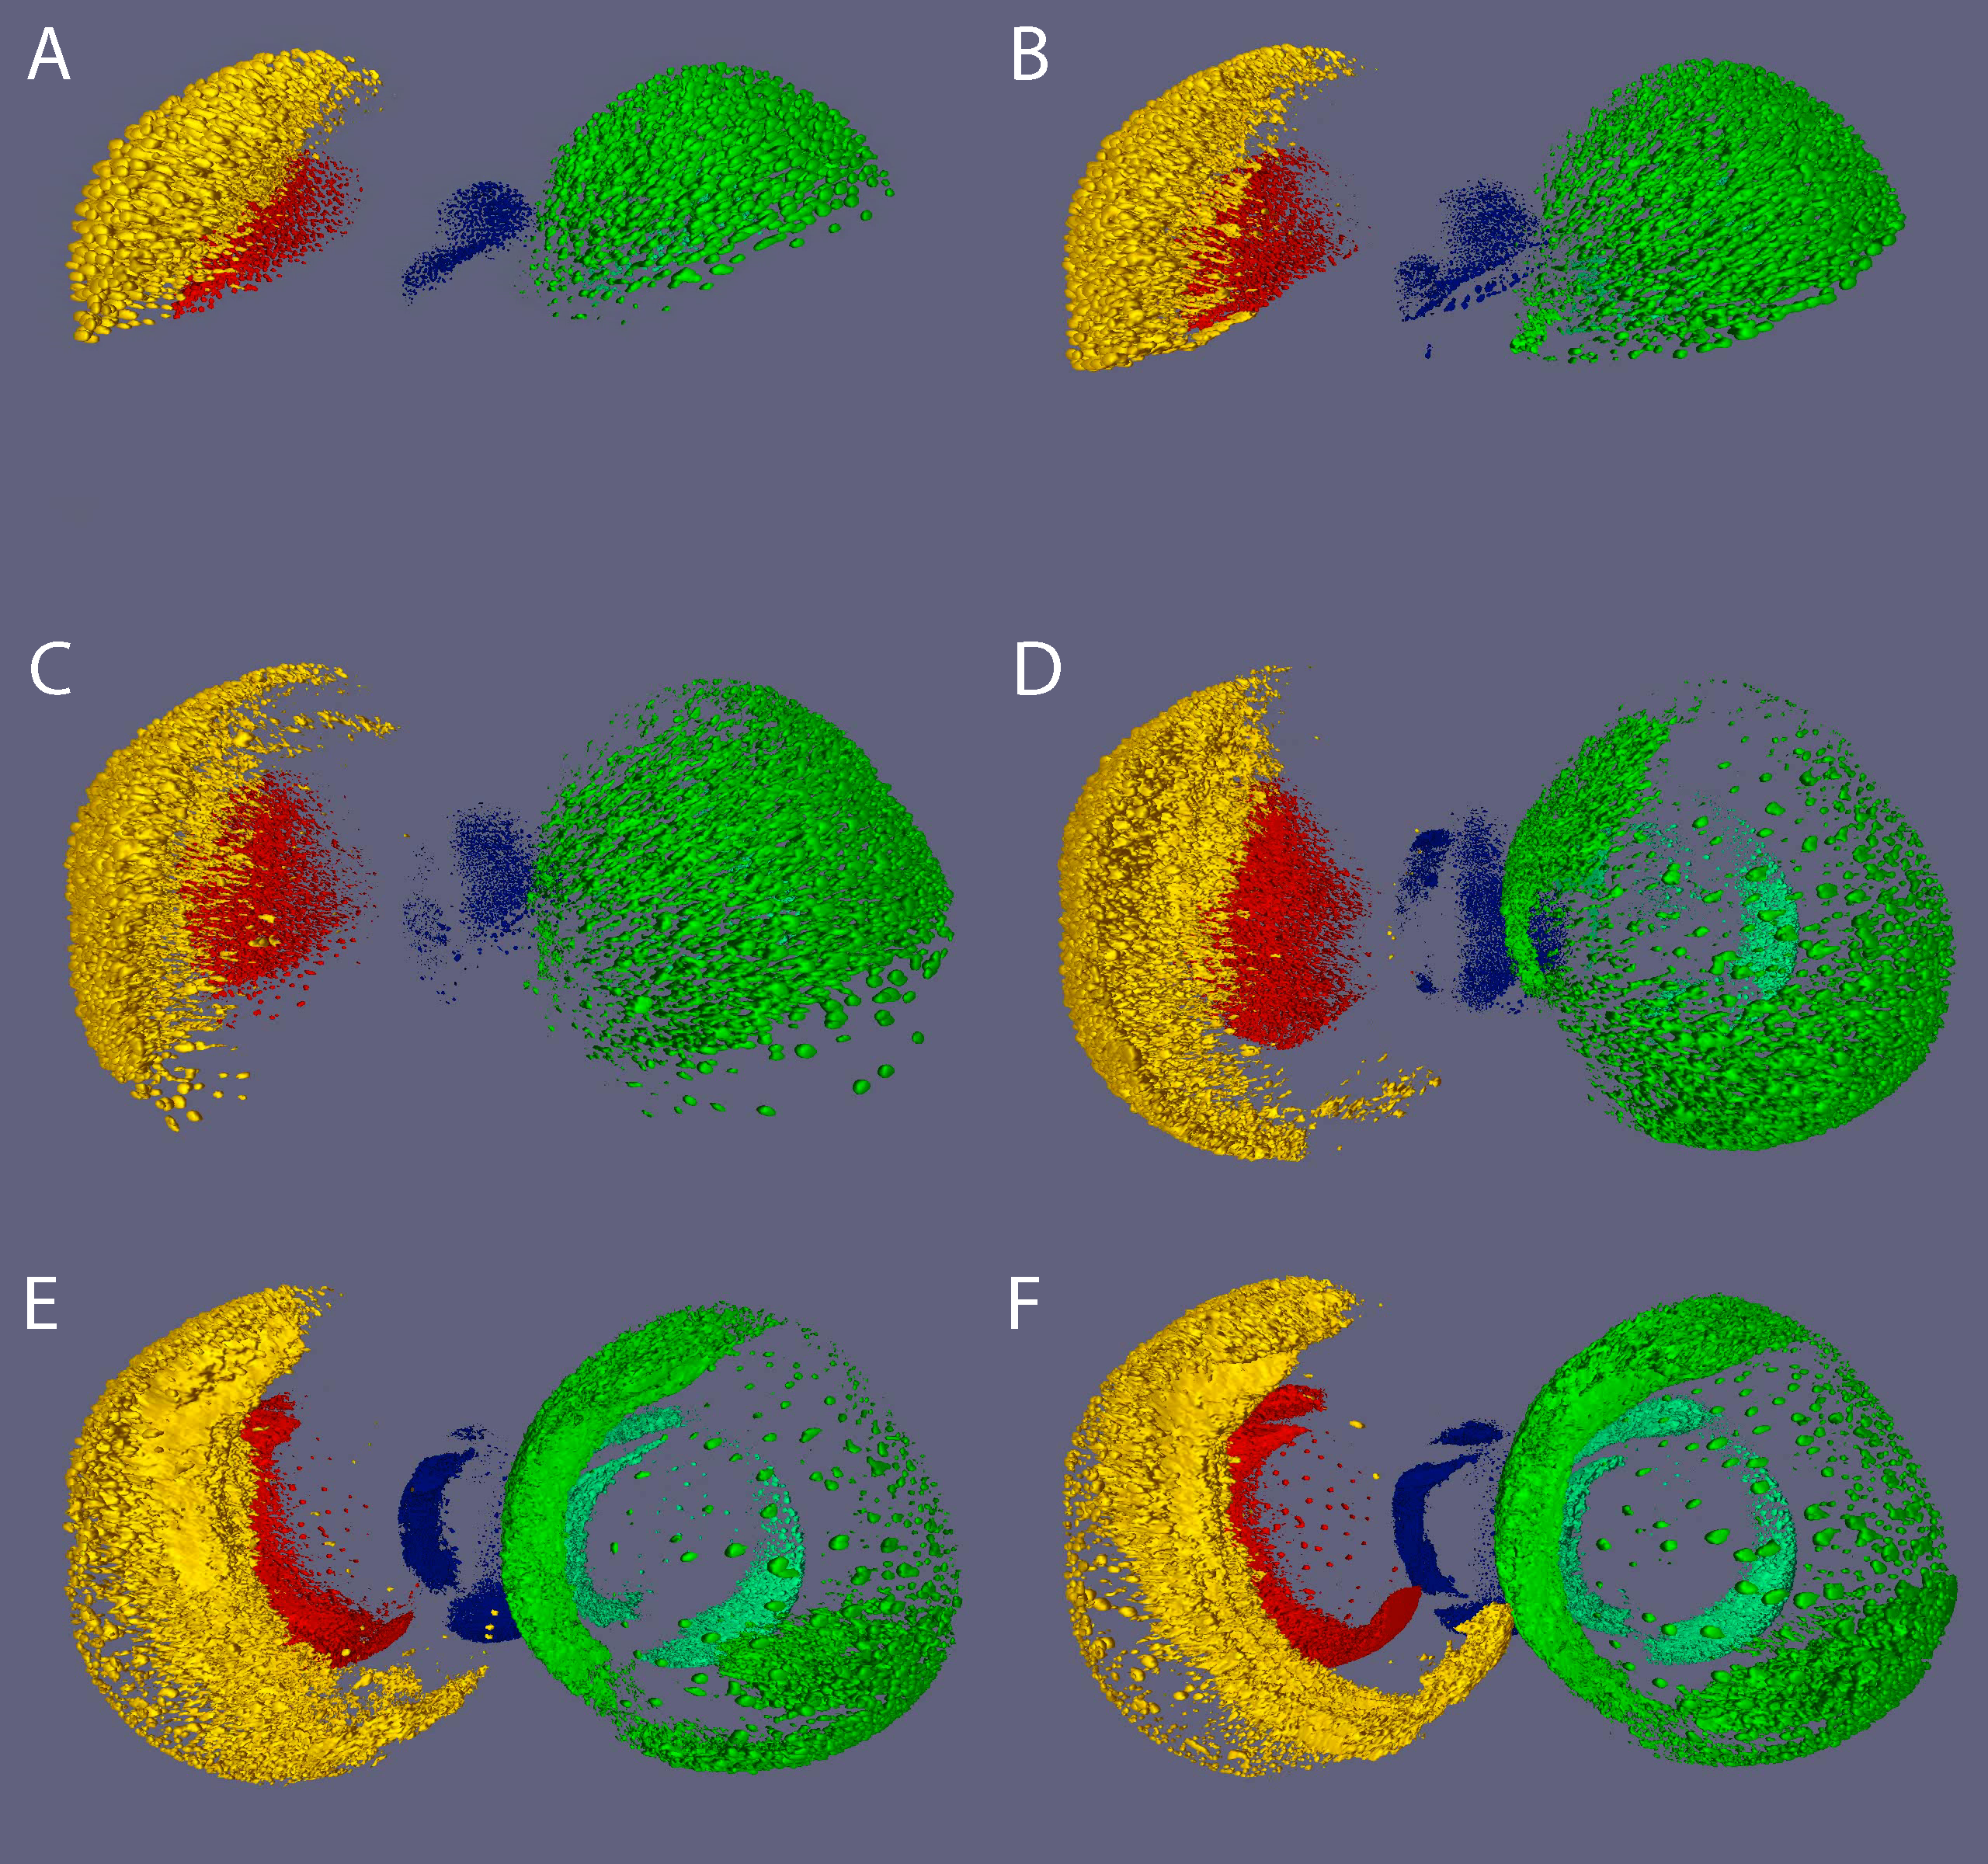
\includegraphics[width=0.9\textwidth]{../../images/Reconstruction/washington/5angles_before_letter.png}
\end{center}
\caption{\textbf{Original five views produced by the Digital Scanning Light Microscope (DSLM).} Isosurfaces have been extracted from the DSLM raw data. Each view is obtained by rotating the embryo 72 degrees (one color per angle of view). A: Sphere stage. B: 40 percent epiboly. C: 75 percent epiboly. D: 90 percent epiboly. E: 8-somite stage. F: 12-somite stage.}
\label{washington_5angles_before}
\end{figure}

\subsubsection{Manual Registration  }
\begin{figure}
\begin{center}
\includegraphics[width=0.6\textwidth]{../../images/Reconstruction/washington/workflow_manual_corrected.png}
\end{center}
\caption{\textbf{The manual registration component.} This process aims at inferring the parameters required for a spatial registration of the five angles of view. }
\label{washington_workflow_manual}
\end{figure}

   We explain here the manual registration component (Fig. \ref{washington_workflow_manual}). The DSLM allows rapid imaging of the embryo and, coupled with a rotating device, recording multiple views of the same embryo obtained from different angles (Fig. \ref{washington_SPIM}). We have been using an exact replicate of the DSLM described in \cite{Keller:2008km}. In this whole section 7.2, we use the following conventions to name the axes of each view: the axis from the camera to the embryo is the z-axis or "depth", the horizontal axis of the light plane is the x-axis, and the vertical axis of the light plane is the y-axis.  
\begin{figure}
\begin{center}
\includegraphics[width=0.9\textwidth]{../../images/Reconstruction/washington/SPIM_corrected.png}
\end{center}
\caption{\textbf{Digital Scanning Light Microscope (DSLM) setup.} Diagram after P.J. Keller, E. Stelzer et al. \cite{Keller:2008km}, adapted by V. Gurchenkov.}
\label{washington_SPIM}
\end{figure}

   Reconstructing an \textit{in toto} view of the embryo requires the spatial fusion of the five views within a reference frame. While sophisticated methods of non-rigid spatial registration based on raw image processing and "wavelets" are currently being developed by our team \cite{RubioGuivernau:2012dx}, we decided to design our own. Here, we rely on the knowledge of the rotating motion of the microscope plate to geometrically infer a rigid spatial registration. Moreover, we assume that the registration parameters remain constant throughout the imaging process since the embryo is not moving in the agarose chamber and the rotating plate executes precise and controlled displacements. Thus we use a single time step to calculate the parameters, which will be generalized to all other time steps.  

   The embryo is mounted onto a cylindrical agarose tube. The tube is fixed on a table that can rotate around the cylinder's central axis and translate it. As the embryo never passes exactly through that central axis, the software controlling the motion of the table must be calibrated before the time-lapse imaging starts. The calibration phase is equivalent to the following process (Fig. \ref{washington_manual_spim}): the operator must center the embryo in the light plane. Once the position is validated, the software performs a 90 degree rotation and the operator must center again the embryo in the light plane. Based on the translation vector created by the operator's action, the software computes the relative position of the embryo with respect to the cylinder's center. However, the computed relative position is only an approximation of the real relative position because the operator's estimation is never exact. This is due to the fact that s/he only sees a projection along the z-axis, and as the embryo rotates, the aspect on the screen changes.  
\begin{figure}
\begin{center}
\includegraphics[width=0.9\textwidth]{../../images/Reconstruction/washington/manual_spim.png}
\end{center}
\caption{\textbf{Schema of the calibration phase. } Left: The operator centers the embryo in the light plane. Right: To decipher the relative position of the embryo with respect to the center of rotation, the software performs a 90 degree rotation, then the operator must translate the embryo back into the light plane (blue vector). }
\label{washington_manual_spim}
\end{figure}

   We have programmed a graphical user interface to manually correct the estimation error and determine the optimal relative position (Fig. \ref{washington_manual_registration_selection}). The two parameters controlled by the user are the coordinates of the correction vector. As the user moves this vector, s/he can directly observe the motion of the five views computed in real time, hence determine the optimal correction vector. For this task, the nuclei of the margin (yolk syncytial layer), which are separated from the mass of the deep cells, offer useful landmarks for a precise determination of these vector coordinates, i.e. the best match (Fig. \ref{washington_manual_registration_final}).  
\begin{figure}
\begin{center}
\includegraphics[width=0.9\textwidth]{../../images/Reconstruction/washington/manual_registration_selection.png}
\end{center}
\caption{\textbf{Graphical user interface designed to infer the estimation of the center of rotation.} The red line passes through the center of rotation determined by the calibration phase. The brown line passes through the corrected center of rotation. As the user moves the brown line, the five angles of views are repositioned in real time, allowing to infer the best estimation of the center of rotation.}
\label{washington_manual_registration_selection}
\end{figure}
\begin{figure}
\begin{center}
\includegraphics[width=0.9\textwidth]{../../images/Reconstruction/washington/manual_registration_final.png}
\end{center}
\caption{\textbf{Best match for the rigid manual registration. } The marginal yolk nuclei visible on top of the embryo are used to estimate the correct registration parameters. }
\label{washington_manual_registration_final}
\end{figure}

   After the five views have been registered for one time step, the same registration parameters will be applied to the whole time lapse imaging data in the other components of the workflow (Fig. \ref{washington_workflow}). However, as it can be noticed in Fig. \ref{washington_5angles_after}, the optical deformation induced by the perturbation of the light path through the embryonic tissue causes the result to be rather suboptimal. Other components of the workflow (Voxel Quality Evaluation and Blending Function) will take care of removing these defects in each view.  
\begin{figure}
\begin{center}
\includegraphics[width=0.9\textwidth]{../../images/Reconstruction/washington/5angles_after_letter.png}
\end{center}
\caption{\textbf{The five DSLM views superimposed by rigid registration.} These views are identical to the ones shown in Fig. \ref{washington_5angles_before}. A: Sphere stage. B: 40 percent epiboly. C: 75 percent epiboly. D: 90 percent epiboly. E: 8-somite stage. F: 12-somite stage.}
\label{washington_5angles_after}
\end{figure}

\subsubsection{Voxel Quality Evaluation  }
\begin{figure}
\begin{center}
\includegraphics[width=0.6\textwidth]{../../images/Reconstruction/washington/workflow_vqe_corrected.png}
\end{center}
\caption{\textbf{The voxel quality component.} This process aims at quantitatively evaluating the local image quality for each angle of view. }
\label{washington_workflow_vqe}
\end{figure}

   The voxel quality component runs independently from the manual registration component. Its goal is to determine what spatial region of the volume shows the best signal quality, in each view and at every time step. The actual output of this component is to attribute a quality score to each voxel of the volume. The rationale here is that the farther the light travels through the embryo, the more degraded the signal is. The light beam through the embryo is split into two orthogonal beams: the continuation of the original light beam from the laser, and a new light beam emitted by the fluorescent molecules of the embryo toward the camera. For the voxel quality component, the relevant part of the light beam is inside the embryo. We performed a geometrical computation to determine the length of the light beam from each voxel of the volume to the physical border of the embryo. For the evaluation, we first calculated the border and then the beam length. It can be summarized as follows:  
\begin{itemize}
	\item 1. To eliminate the low amplitude background noise, the averaged voxel intensity of the volume was computed to determine the isosurface of the nuclei's shapes (Fig. \ref{washington_vqe}A). This isosurface is a mesh of triangles. 
	\item 2. After a random decimation of the isosurface triangles to decrease the number of vertices, small spheres were centered on these vertices and resized in order to produce a contiguous embryo surface without holes. Then, a binary mask of the image was extracted to store the outer shape of the embryo.
	\item 3. We eliminated spurious signal traces (blue arrows in Fig. \ref{washington_vqe}B) that may have subsisted outside of the embryo shape by keeping only the closed region that had the largest volume.
	\item 4. The spheres creating an embryo larger than desired, we eroded the volume by an amount equivalent to the radius of the spheres to obtain the actual physical border of the embryo. The reduced volume is stored as a binary data array with value 1 (resp. 0) for voxels inside (resp. outside) the border (Fig. \ref{washington_vqe}C).
	\item 5. Since each view is oriented with its z-axis along the camera path and x-axis along the illumination plane, it is now straightforward to compute both distances from the border by counting the number of 1's along those axes (Fig. \ref{washington_vqe}D,E). The voxels that are outside of the border receive an eliminatory score as they cannot be used for the registration task (Fig. \ref{washington_vqe}F).
	\item 6. Finally, we also eliminated the voxels located beyond a cutoff distance (about 200$\mu$m) in both directions as they belonged to parts of the image that were too degraded to be used (Fig. \ref{washington_vqe}G,H,I).
\end{itemize}
\begin{figure}
\begin{center}
\includegraphics[width=0.9\textwidth]{../../images/Reconstruction/washington/vqe_letter.png}
\end{center}
\caption{\textbf{The various steps of the voxel quality evaluation component.} See text.}
\label{washington_vqe}
\end{figure}

\subsubsection{Blending Function  }
\begin{figure}
\begin{center}
\includegraphics[width=0.6\textwidth]{../../images/Reconstruction/washington/workflow_blend_corrected.png}
\end{center}
\caption{\textbf{The blending function component.} This component builds a function determining what original angle of view has the best quality score for each voxel in the registered space.}
\label{washington_workflow_blend}
\end{figure}

   The objective of this task is to use both the manual registration component and the voxel quality evaluation component described in the previous subsections to build a blending function. For each registered voxel, this function selects among all five views which one will be used in the \textit{in toto} reconstruction. In other words, the blending function produces a 3D integer volume in which each voxel contains the id of the most relevant angle of view according to its quality evaluation. Knowing the coordinates of the center of rotation, we were able to precisely position all five views within a common reference space (Fig. \ref{Reconstruction_5angles_3Dvolume}, left). In this space, we visited each voxel and checked for each projected angle of view whether it was located inside the embryo border evaluated in the previous component (Fig. \ref{Reconstruction_5angles_3Dvolume}, right). Then, we attributed to this voxel the id of the angle of view (from 1 to 5) under which it had the best quality, or 0 if it was lying outside of all borders. This produced the integer mask shown in Fig. \ref{washington_blendingfunction}. Note that instead of the maximum voxel quality, we could also have used a weighted average of all angles. An output of the blending function applied to the raw voxel intensities is shown in Fig. \ref{washington_blendingfunction_raw}, providing a first example of \textit{in toto} registration of the embryo. In our workflow, however, we applied the blending function to the "deformation fields" calculated in the next component.  
\begin{figure}
\begin{center}
\includegraphics[width=0.9\textwidth]{../../images/Reconstruction/5angles_fusion.png}
\end{center}
\caption{\textbf{Relative positions of the five views in the registered space.} Left: The five cubes represent the original reference frames of the five different views. Right: A 2D illustration of the sequential visit of the registered voxels.}
\label{Reconstruction_5angles_3Dvolume}
\end{figure}
\begin{figure}
\begin{center}
\includegraphics[width=0.9\textwidth]{../../images/Reconstruction/washington/blendingfunction.png}
\end{center}
\caption{\textbf{Five-valued blending function mask.} In the registered space, the color of each voxel represents the id of the original angle of view under which it has the best quality. }
\label{washington_blendingfunction}
\end{figure}
\begin{figure}
\begin{center}
\includegraphics[width=0.9\textwidth]{../../images/Reconstruction/washington/blendingfunction_raw.png}
\end{center}
\caption{\textbf{Output of the blending function applied to the raw voxel intensities.}}
\label{washington_blendingfunction_raw}
\end{figure}

\subsubsection{Deformation Fields  }
\begin{figure}
\begin{center}
\includegraphics[width=0.6\textwidth]{../../images/Reconstruction/washington/workflow_deffield_corrected.png}
\end{center}
\caption{\textbf{The deformation field component.} This component produces a 3D vector field that indicates the direction and amplitude of local displacements in each voxel.}
\label{washington_workflow_deffield}
\end{figure}

   The objective of the deformation field component is to reconstruct the spatial deformation that relates two 3D volumes produced by the DSLM at consecutive time steps under the same angle of view (one of the five; Fig. \ref{washington_vueGlobal_frame}), which we denote here by V and V'. The notion of image deformation is close to the notion of optical flow as its goal is to compute the image motion between consecutive images. We employed a non-rigid registration method called "Demons Registration": it acts as if voxel-sized "demons" were pulling and pushing the voxel of volume V' along the local gradient of voxel intensity in volume V. This method is iterative and the demons run for a predefined number of steps, or until some matching criterion is reached. The implementation that we used here is based on Thirion's algorithm \cite{Thirion:1998hg}. Fig. \ref{washington_vueDeffield2ts} shows the superposition of the isosurfaces of V (in white) and V' (in yellow) at the marginal region of the zebrafish embryo. As the deformation field was computed in the entire images of V and V', and not only at the position of the nuclei, we had to filter out spurious vectors from the resulting field. The vectors belonging to voxels located inside the nucleus envelopes (corresponding to another isosurface obtained by thresholding the voxels at twice the mean volume intensity) were retained, while the others were nullified. We calculated the deformation fields for each angle of view separately. The next component takes care of blending them together.  
\begin{figure}
\begin{center}
\includegraphics[width=0.9\textwidth]{../../images/Reconstruction/washington/deffield/vueGlobal_frame.png}
\end{center}
\caption{\textbf{One volume V under one of the five angles of view.} The white grains represent the envelopes of the nuclei calculated by thresholding the voxels at twice the mean intensity of V.}
\label{washington_vueGlobal_frame}
\end{figure}
\begin{figure}
\begin{center}
\includegraphics[width=0.9\textwidth]{../../images/Reconstruction/washington/deffield/vueDeffield2ts.png}
\end{center}
\caption{\textbf{Deformation field between two volumes V and V' at consecutive time steps.} The white isosurface represents V, the yellow isosurface represents V'. Not all deformation arrows are displayed.}
\label{washington_vueDeffield2ts}
\end{figure}

\subsubsection{Blended Deformation Fields  }
\begin{figure}
\begin{center}
\includegraphics[width=0.6\textwidth]{../../images/Reconstruction/washington/workflow_blend_deffield_corrected.png}
\end{center}
\caption{\textbf{The blended deformation field component.} This component combines the blending function with the 3D deformation vector field.}
\label{washington_workflow_blend_deffield}
\end{figure}

   Finally, the blending function obtained in Section 7.2.3 is applied to the five deformation vector fields obtained in Section 7.2.4. Each voxel of the reference volume simply receives the deformation vector from the angle of view that has the best quality evaluation score.  
\begin{figure}
\begin{center}
\includegraphics[width=0.9\textwidth]{../../images/Reconstruction/washington/blendingfunction_deffield.png}
\end{center}
\caption{\textbf{Blended deformation field at a given time step viewed from four different angles.} (Note that these angles do not correspond to the original angles of view.)}
\label{washington_blendingfunction_deffield}
\end{figure}
\begin{figure}
\begin{center}
\includegraphics[width=0.9\textwidth]{../../images/Reconstruction/washington/blendingfunction_deffield_multits.png}
\end{center}
\caption{\textbf{Blended deformation field at successive time steps viewed from the same angle.}}
\label{washington_blendingfunction_deffield_multits}
\end{figure}
